\section{Search Strategies}
\label{sec:technical}

\begin{figure}
    \begin{center}
        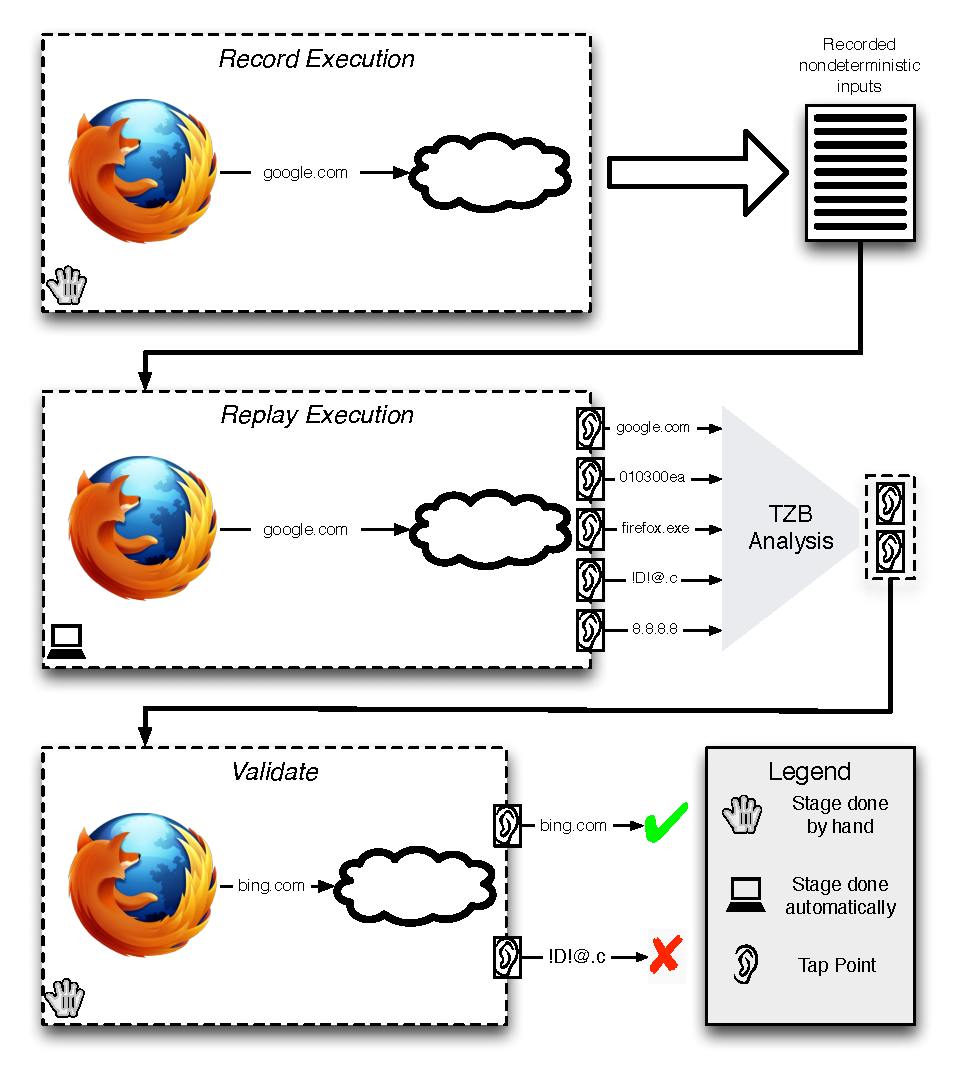
\includegraphics[width=3.2in]{figures/tzbarch.pdf}
    \end{center}
    \caption{The workflow for using TZB to locate points at which to
    interpose for active monitoring.}
    \label{fig:workflow}
\end{figure}

To find useful \emph{tap points} in a system---places from which to
extract data for introspection---using Tappan Zee Bridge, one begins by
creating a recording that captures the desired OS or application
behavior. For example, if the end goal is to be notified each time a
user loads a new URL in Firefox, one would create a recording of Firefox
visiting several URLs. This recording is made by emulating the OS and
application inside of TZB, which can capture and record all sources of
non-determinism with low overhead, allowing for later deterministic
replay. Next, one can run one or more analyses that seek out the desired
information among all memory accesses seen during the execution.
Analyses in TZB take the form of PANDA plugins that are called on each
memory access made during a replayed execution and, at the end, write
out a report on the tap points analyzed. Finally, the tap points found
should be validated to ensure that they do, in fact, provide the desired
information. Such assurance can be gained either by examining the data
in the tap point in new executions, or by examining the code around the
tap point. This workflow is illustrated in Figure~\ref{fig:workflow}.

In this section, we describe three different ways of finding tap points
grouped according to a standard epistemic classification
scheme~\cite{Rumsfeld:2002}: searching for ``known knowns''---tap points
where the desired data and its format is known; searching for ``known
unknowns''---tap points where the kind of data sought is known, but its
precise format is not; and finally ``unknown unknowns''---tap points
where the type and format of the data sought are not known, and we are
instead simply trying to find ``interesting'' tap points.

\subsection{Known Knowns}

The simplest case is finding data that one knows is likely to be read or
written by a tap point, and where the encoding of the data is easily
guessed. For example, to find a tap point that can be used to notify
the hypervisor whenever a URL is entered in a browser, one can visit a
known sequence of URLs, and then monitor all tap points, searching for
specific byte sequences that make up those URLs. The same holds for
other data whose representation when written to memory is predictable:
filenames, window titles, registry key names, and so on. For this kind
of data, simple string searching is usually sufficient to zero in on the
few tap points that handle the data of interest, and in our experience
it is one of the most effective techniques for finding useful tap
points.

\subsection{Known Unknowns}
\label{sec:technical:subsec:knownunk}

A second tap point application involves finding tap points for things
about which we have limited knowledge.

We can easily assemble corpora of exemplars to represent a semantic
class: English prose, kernel messages, or mail headers. These examples
need not come from tap points but can easily be collected directly from
interacting with the operating system itself. From such a corpus, we can
readily build a statistical model of the semantic class. Tap points
whose contents have high likelihood ratios for the semantic model with
respect to a null model are likely to come from the same semantic class
as the corpus. This kind of supervised learning permits us, for
instance, to train a model on examples of the contents of \texttt{dmesg}
under Linux and employ it to locate tap points that write analogous data
in other operating systems such as FreeBSD, Minix, and Haiku.

In addition to statistical comparison to a known exemplar, we can also
search for data of unknown format if we have access to some external
validator. This is the case, for example, when searching for tap points
that write encryption keys: although the exact key may not be known in
advance (ruling out the use of string matching), if we have bit of
encrypted data we can check whether a given byte string is a valid
decryption key by trying to decrypt our sample data.

\subsection{Unknown Unknowns}

The final strategy for finding useful tap points is also the least
focused. If there is no specific introspection quantity sought, one
might instead wish to find interesting tap points, for some suitable
definition of ``interesting.'' To support this scenario, TZB offers a
form of unsupervised learning---clustering---to group together tap
points that handle similar data. The idea is that one can then examine
exemplars from each cluster, rather than being forced to look through a
large number of tap points. Thus, our use of clustering functions as a
form of \emph{data triage}.
